\section{Introduction}

The ring loading problem first arose in the planning of \textbf{S}ynchronous \textbf{O}ptical \textbf{Net}working (SONET) rings.
In SONET, several add-drop multiplexers (ADMs) and other components are connected by predominantly optical fibers.
One prominent SONET topology is the bidirectional path-switched ring, which is safe to the failure of a single link or node due to its connectivity.
In a SONET ring, the routing of node-to-node network traffic is fixed: Unless a failure occurs, the traffic between any two nodes is either always routed in the clockwise or the counter-clockwise direction.
The ring loading problem arises in the planning of such rings.
ADMs have a limited capacity of traffic they can send or receive through any link.
Hence the maximal workload on any link must be determined from estimated node-to-node network traffic demands during planning.
This involves computing the optimal routing of these demands around the ring, that is, the routing that minimizes the maximal load on any link.
As it turns out, determining such a routing is quite difficult.

In the paper "The Ring Loading Problem" from 1999, the authors Schrijver, Seymour and Winkler~\cite{schrijver99} derived an approximation algorithm for the ring loading problem.
In this work parts of this paper are presented.

We begin by formalizing the problem.
The SONET ring is modeled by an undirected cycle graph consisting of $n \in \N$ nodes.
We number the nodes consecutively in the counter-clockwise direction with the numbers $1, 2, \dots, n$.
For the ease of notation, we also refer to node $1$ as node $n+1$.
This means that we can write the edge set as $E = \{\{i, i+1\}\ |\ i \in [n]\}$, where $[n] \coloneqq \{1, 2, \ldots, n\}$.
Now, for every two nodes $i \neq j$ we are given a (traffic) demand $d_{i, j} \in \R_{\geq 0}$, which represents the network traffic that has to be routed from node $i$ to node $j$ (hence we call the commodity that is being routed "traffic").
For simpler notation, we only allow one demand per pair of nodes.
As we will see, this does not oversimplify the problem.
Also, \citet{schrijver99} claim that their algorithm can be easily extended to the case of two (or more) demands per pair.
Thus, we focus on the case where for every two nodes $i < j$, we have one demand $d_{i,j}$.

A demand $d_{i, j}$ can be routed two ways around the ring.
We say that a demand is routed \emph{forward} or \emph{through the front}, if it does not use the edge $\{n, 1\}$.
Otherwise, we say that the demand is routed \emph{backwards} or \emph{through the back}.
Next, we can formally define routings.
\begin{definition}[Routing]
	\label{def:routing}
	A \emph{real-valued routing} in a ring of size $n \in \N$ is a function 
	\begin{equation}
		\Phi: \{(i, j)\ | \ i, j \in [n], i < j\} \rightarrow [0, 1] \ .
	\end{equation}
	A \emph{binary routing} is a real routing $\Phi$ which only takes values in $\{0, 1\}$. 
\end{definition}
We interpret the value $\Phi(i, j)$ as the fraction of the demand $d_{i, j}$ that is routed through the front.
If $\Phi(i, j) \in (0, 1)$ holds, we say that $\Phi$ \emph{splits} the demand $d_{i, j}$.

\begin{definition}[Edge load, Ringload]
	\label{def:edge-load}
	Let $\Phi$ be a (real-valued) routing.
	For every edge $\{k, k+1\}$, $k \in [n]$, we define the \emph{edge load} $L_k(\Phi)$ as the total traffic that is routed through that edge:
	\begin{equation}
		\label{eq:edge-load}
		L_k(\Phi) \coloneqq \sum_{\substack{1 \leq i < j \leq n,\\ k \in [i, j)}} d_{i, j} \Phi(i, j) + \sum_{\substack{1 \leq i < j \leq n,\\ k \notin [i, j)}} d_{i, j} (1 - \Phi(i, j)) \ .
	\end{equation}
	The \emph{ringload} $L(\Phi)$ is the maximal edge load under the routing $\Phi$.
\end{definition}
Observe that in \cref{def:edge-load}, we have $k \in [i, j)$ if and only if the edge $\{k, k+1\}$ lies on the front route of the demand $d_{i, j}$.

With these preparations, we can now formulate the ring loading problem in mathematical terms:
\begin{center}
	\begin{mdframed}
		\centering
		\textsc{RingLoading}\\[0.7em]
		\begin{tabular}{rl}
			{\bfseries Input}: & Ring size $n \in \N, n > 1$ and demands $d_{i, j} \in \R_{\geq 0}$ for all $1 \leq i<j\leq n$.\\
			{\bfseries Output}: & Binary routing $\Phi$ that minimizes $L(\Phi) = \max_{i \in [n]} L_i(\Phi)$.
		\end{tabular}
	\end{mdframed}
\end{center}
We can encode an instance of \RL in $\cO(K \log D + \log n)$ space, where $K \in \N$ is the number of non-zero demands and $D = \max_{1 \leq i < j \leq n}d_{i, j}$ the maximal demand.
In general, we have $K \in \cO(n^2)$.

As mentioned above, determining the optimal ringload of any \RL instance is quite difficult.
If we formulate \RL as a decision problem, by asking
\begin{quote}
	"Given an instance of \RL and $T \in \N$, does there exist a binary routing $\Phi$ with ringload $L(\Phi) \leq T$?",
\end{quote}
the problem is NP-complete.
\begin{theorem}
	\RL in its decision form is NP-complete.
\end{theorem}
\begin{proof}[Proof (Sketch)]
	A routing $\Phi$ restricted to the non-zero demands serves as a witness of size $\cO(K)$.
	Using \cref{eq:edge-load} we can determine the maximal edge load $L(\Phi)$ in polynomial time and check whether $L(\Phi) \leq T$.
	Thus, \RL is in NP.
	
	To show completeness, we follow the proof given in \cite{schrijver99} and reduce \textsc{Partition} \cite{karp72}.
	This problem asks whether, given an instance $J$ consisting of $m$ positive integers $\{z_1, \ldots, z_m\} \subset \N$, there exists a subset $S \subseteq [m]$ that fulfills
	\begin{equation}
		\sum_{i \in S} z_i = \frac{1}{2}  \sum_{i \in [m]} z_i = \sum_{j \in [m] \setminus S} z_j\ .
	\end{equation}
	We construct a \RL instance $J'$ of size $m + 3$ with the following demands:
	\begin{align}
			d_{i, m+2} &\coloneqq z_i \quad \forall i \in [m], \\
			d_{m, m+1} &\coloneqq d_{m+1, m+2} \coloneqq \frac{1}{2}  \sum_{i \in [m]} z_i \ . 
	\end{align}
	All other demands are set to $0$.
	Furthermore, we set $T \coloneqq \sum_{i \in [m]} z_i$.
	The constructed instance is visualized in \cref{fig:partition-rl-instance}.
	
	Now, assume that $J$ is a Yes-instance of \textsc{Partition}.
	Then there exists a solution $A \subseteq [m]$.
	Consider the binary routing
	\begin{align}
		\Phi(i, m+2) &= 1 \quad \forall i \in A \ , \\
		\Phi(i, m+2) &= 0 \quad \forall i \in [m] \setminus A \ ,	 \\
		\Phi(m+1, m+2) & = \Phi(m+2, m+3) = 1 \ .
	\end{align}
	We observe that $L_i \leq T$ for all $i \in [m] \cup \{m+3\}$ and that $L_{m+1} = L_{m+2} = T$.
%	The loads $L_{m+1}, L_{m+2}$ are
%	\begin{equation}
%		L_{m+1} = \frac{1}{2} \sum_{i \in S} z_i + \sum_{i \in A} z_i 
%		= T
%		= \frac{1}{2} \sum_{i \in S} z_i + \sum_{i \in [m] \setminus A} z_i 
%		= L_{m+2} \ .
%	\end{equation}
	This implies $L(\Phi) = T$ and thus the constructed instance is a Yes-instance of \RL.
	
	Similarly, it can be shown that if $J'$ is a Yes-instance with routing $\Phi$, the set 
	\begin{equation}
		A' \coloneqq \{i \ |\ i \in [m] \text{ and } \Phi(i, m+2) = 1\}
	\end{equation} 
	is a solution to the \textsc{Partition} instance $J$.
	This shows NP-completeness.
%	In fact, the routing $\Phi$ is the only routing with ringload $\leq T$ in $J'$.
%	To see this, let $\Phi'$ be another routing and assume that any of the demands $d_{m+1, m+2}, d_{m+2, m+3}$ is routed backwards, w.l.o.g. $d_{m+1, m+2}$.
%	Then we have
%	\begin{equation}
%		L_{m+2}(\Phi) \geq d_{m+2, m+3} + d_{m+1, m+2}  
%		= \frac{1}{2} \sum_{i \in S} z_i + \frac{1}{2} \sum_{i \in S} z_i 
%		= T \ .
%	\end{equation}
%	Now, no other demand can be routed through the edge $\{m+2, m+3\}$
\end{proof}

\begin{figure}
	\centering
	\begin{minipage}[t]{.4\textwidth}
		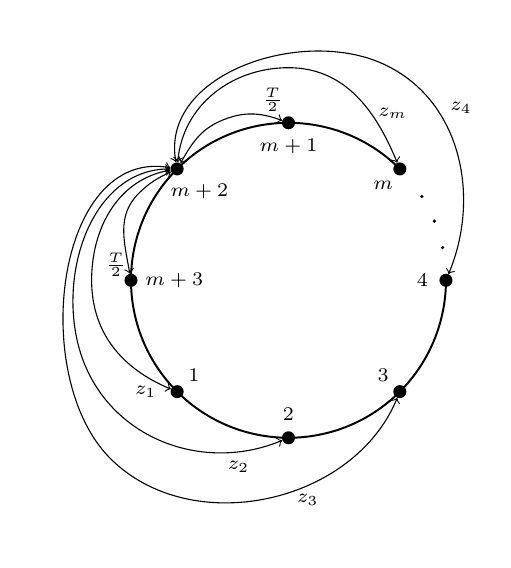
\begin{tikzpicture}[font=\scriptsize, node/.style={circle,thick,draw},
		l_2/.style={line width =0.25mm},
		scale=1, transform shape]
		% equidistant points and arc
		\foreach \x [count=\p] in {0,...,7} {
			\node[shape=circle,fill=black, scale=0.5] (\p) at (\x*45-135:2) {};
		};
		\foreach \x [count=\p] in {0,...,3} {
			\draw (225 + \x*45:1.7) node {\p};
			%				\draw (-30-\x*60:2.4) node {$\bar{\p}$};
		}; 
		\draw (225 + 4*45:1.7) node {$m$};
		\draw (225 + 5*45:1.7) node {$m+1$};
		\draw (225 + 6*45:1.6) node {$m+2$};
		\draw (225 + 7*45:1.45) node {$m+3$};
		
		\draw[l_2] (5) arc (45:360:2);
		\draw[line width =1.3pt, line cap=round, dash pattern=on 0pt off 10pt] (12:2) arc(12:35:2);
		

		\draw[<->] (1)  to [out=157.5,in=-90] (180:2.5) to [out=90,in=-170](7);
		\draw[<->] (2)  to [out=-157.5,in=-67.5] (-157.5:2.8) to [out=112.5,in=-180] (7);
		\draw[<->] (3)  to [out=-112.5,in=-45] (-135:3.2) to [out=135,in=-190] (7);
		\draw[<->] (4)  to [out=67.5,in=-22.5] (67.5:3) to [out=157.5,in=100] (7);
		\draw[<->] (5)  to [out=112.5,in=0] (90:2.7) to [out=180,in=85] (7);
		
		\draw[<->] (6)  to [out=160,in=22.5] (112.5:2.2) to [out=-157.5,in=60] (7);
		\draw[<->] (8)  to [out=100,in=-135] (150:2.2) to [out=45,in=-155] (7);
		
		\node (a) at (-142:2.3) {$z_1$};
		\node (b) at (-105:2.45) {$z_2$};
		\node (c) at (-85:2.8) {$z_3$};
		\node (d) at (45:3.1) {$z_4$};
		\node (e) at (58:2.5) {$z_m$};
		\node (d) at (95:2.3) {$\frac{T}{2}$};
		\node (f) at (175:2.2) {$\frac{T}{2}$};
%		\node (bottom) at (0, -2.8) {};
		%		\draw[dashed] (1) -- (3) -- (5) -- (1);
		% axes
		%		\draw [dotted, gray] (-2.6,0) -- (2.6,0);
		%		\draw [dotted, gray] (0,-2.15) -- (0,2.15);
		\end{tikzpicture}
	\end{minipage}
	\caption{\RL instance constructed from an instance of \textsc{Partition}.}
	\label{fig:partition-rl-instance}
\end{figure}

The fact hat \RL is NP-complete motivates the search for an approximation algorithm.
One such algorithm was invented by \citet{schrijver99} in the late 1990s.
This algorithm achieves a ringload of $L \leq \Lopt + \frac{3}{2}D$, where $\Lopt$ is the optimal ringload and $D$ the maximal demand.
The idea is to first solve the following problem.
\begin{center}
	\begin{mdframed}
		\centering
		\textsc{RelaxedRingLoading} (\textsc{RRL})\\[0.7em]
		\begin{tabular}{rl}
			{\bfseries Input}: & Ring size $n \in \N, n > 1$ and demands $d_{i, j} \in \R_{\geq 0}$ for all $1 \leq i<j\leq n$.\\
			{\bfseries Output}: & Real-valued routing $\Phi$ that minimizes $L(\Phi) = \max_{i \in [n]} L_i(\Phi)$.
		\end{tabular}
	\end{mdframed}
\end{center}
In contrast to \RL, this problem can be solved in polynomial time, as it can also be formulated as a linear program.
We will see in \cref{sec:relaxed-ring-loading} that \RRL always has optimal solutions in which at most $\lfloor \frac{n}{2} \rfloor$ demands are routed both ways around the ring.
From such a routing an approximation of an optimal binary routing can be easily obtained, as will be shown in \cref{sec:ring-loading}.

%In this work, Schrijver et al.'s algorithm is presented and its correctness proven.
%This involves two steps: First, deriving an algorithm for computing an optimal real-valued routing and second, transforming it into a binary routing.

%\citet{schrijver99} claim that their algorithm has a time-complexity of $O(k n^2)$, where $k$ is the number of non-zero demands.
%In this work, I show that through the use of dynamic programming and some modification the complexity can be reduced to $\cO(n^2)$, which seems to be a novel result.
%This runtime is almost optimal, since in the worst case $k = \binom{n}{2} \in \Theta(n^2)$.
%The improved time-complexity is interesting for several reasons:
%\begin{itemize}
%	\item The best currently known runtime for computing an $\Lopt + \frac{3}{2}D$ approximation to \RL is $O(k n^2)$.
%	The proposed modifications improve this runtime by a factor of $k$.
%	\item The best currently known runtime for solving \RRL is $O(k + t_k)$ for integer demands \cite{wang05}, where $t_k$ is the time for sorting $k$ integers and $O(\min\{kn, n^2\})$ \cite{myung04}.
%	The modified algorithm also works for real demands and almost matches the runtime of the latter algorithm.
%	\item Despite the modifications, the algorithm computes the same solution to \RRL as Schrijver et al.'s algorithm, which is particularly aesthetic in the sense that at most $\lfloor\frac{n}{2}\rfloor$ demands are split while the others are routed all front or all back.
%	This means that the runtimes of all algorithms that use Schrijver et al.'s \RRL algorithm as a subroutine are improved as well, in particular that of Schrijver et al.'s approximation algorithm for \RL and that of the PTAS for \RL by \citet{khanna97}.
%\end{itemize}